\section{Mac address hash collisions}

\IEEEPARstart{L}{et} us assume that the MAC address table in an Ethernet switch has the parameters $(n,d)$, where $n$ is the width of the 
address table and $d$ is the depth. Any incoming MAC address is hashed into one of $n$ slots and stored
in one of the $d$ entries. If two different MAC addresses hashes into the same slot we call it a (hash) collision.
 If the slot is already full the switch will replace the oldest entry with the new one. This means that the old value is no longer 
available for making a forwarding descision and whenever a packet arrives destined for this address, the packet
will be forwarded on all ports. So hash collisions leads to flooding.

In the following we will provide some formulae for the probability of flooding as a function of the parameters $(n,d)$ and 
the number of active mac addresses $N$ in the network.

\begin{figure}
\begin{center}
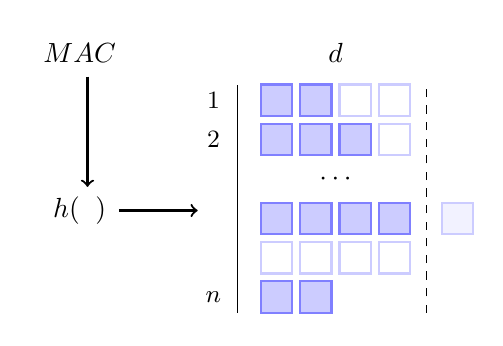
\begin{tikzpicture}
[inner sep=2mm,
box/.style={inner sep=2mm, draw=blue!50,fill=blue!20,thick},
boxe/.style={inner sep=2mm, draw=blue!20, thick},
boxf/.style={inner sep=2mm, draw=blue!20, fill=blue!5, thick}]
\draw ( 1.75 ,3.1) node {$d$};
\draw (-1.5, 3.1) node {$MAC$};
\draw (-1.5, 1.1) node {$h( \; \; )$};
\draw [->, thick] (-1.4, 2.8) to (-1.4, 1.4);
\draw [->, thick] (-1.0, 1.1) to (0.0, 1.1);

\draw (1   ,2.5)     node[box] {};
\draw (1.5,2.5)     node[box] {};
\draw (2.0,2.5)     node[boxe] {};
\draw (2.5,2.5)     node[boxe] {};

\draw (1   ,2.0)     node[box] {};
\draw (1.5,2.0)     node[box] {};
\draw (2.0,2.0)     node[box] {};
\draw (2.5,2.0)     node[boxe] {};

\draw (1.75, 1.5) node {$\cdots$};

\draw (0.2, 2.5) node {\small $1$};
\draw (0.2, 2.0) node {\small $2$};
\draw (0.2, 0.0) node {\small $n$};

\draw (1   ,1.0)     node[box] {};    \draw (1.5,1.0)     node[box] {};     \draw (2.0,1.0)     node[box] {};
\draw (2.5,1.0)     node[box] {};  \draw (3.3,1.0)     node[boxf] {};
\draw (1   ,0.5) node[boxe] {};   \draw (1.5,0.5) node[boxe] {};   \draw (2.0,0.5) node[boxe] {};   \draw (2.5,0.5) node[boxe] {};
\draw (1,   0  ) node[box] {};   \draw (1.5,0) node[box] {};

\draw (0.5,-0.2) to (0.5,2.7);
\draw [dashed] (2.9,-0.2) to (2.9,2.7);
\end{tikzpicture}
\end{center}

\caption{A model of MAC address tables in an Ethernet switch. The table parameters are
$(n,d)$ where $n$ is the number of bins and $d$, the depth,  is the number of entries in each bin.
Any MAC address is hashed into a value from $0$ to $n-1$, and if it is not already in the table it 
is added. If a bin is fully occupied, the oldest entry is discarded.}
\end{figure}


First we assume that MAC addresses are hashed into a uniform distribution. This means that any hash
value is equally probable. The actual distribution of MAC addresses is insignificant as long as the 
hashing function is sufficiently uniform. 
The probability for a MAC address to hash to slot $i$ is thus $p=1/n$. Now we will send $N$ different MAC addresses through
the switch, and
consider the probability for an arbitrary slot $i$ to contain zero, one or more entries after the experiment.
The experiment of hashing a single MAC address and observing wheter it is $i$ or not is called a Bernoulli experiment. 
Each individual Bernoulli experiment is a stochastic
variable $X$ which can have the value 1 if we hash to the value $i$, and 0 if not. 
We now repeate this Bernoulli experiment $N$ times and sums the outcomes to a new stochastic variable $Y$. 

$$
  Y = X_1 + X_2 + \cdots X_N
$$

It is easily shown \cite{Wackerly} that $Y$ is distributed according to the Binomial distribution $\mathbf{B}(N,p)$. 




$$
  Pr\{Y=y\} = \mathbf{B}(N,p) = \binom{N}{n}p^y(1-p)^{N-y}
$$
so the probability that the slot $i$ is empty (Y=0) after $N$ experiments is 
$$
   Pr\{Y=0\} = \binom{N}{0}p^0(1-p)^N = (1-p)^N
$$
if we as an example set $N=8000$ and $n=4096$ we get $(1-1/4096)^{8000} = 14.2\% $.

But how probable is it that all $d$ entries are occupied?
$$
  Pr\{Y>d\} = 1-Pr\{Y\le d\} = 1 - \sum_{y=0}^d Pr\{Y=y\}
$$

$$
  = 1- \sum_{y=0}^d \binom{N}{y} p^y (1-p)^{N-y}
$$

In our case, where $N$ is large and $p$ is small, the Binomial distribution is 
accurately approximated by the Poisson distribution with one parameter $\lambda = Np$.

$$
  Pr(Y=y) = \frac{\lambda^ye^{-\lambda}}{y!}
$$

Following the same arguments as above we get for the probability of all $d$ entries being occupied,

$$
  Pr\{Y > d\} = 1- Pr\{Y\le d \} = 1 - \sum_{y=0}^d Pr\{Y=y\}
$$

$$
 = 1 - \sum_{y=0}^d \frac{\lambda^ye^{-\lambda}}{y!}
$$

As an example of how this is useful consider the table below, where we examine the collision 
probability after exposing the switch to $N=5000$ MAC addresses. For a 16K address table with a depth
of 1 $(16K, 1)$ the probability is 3.81\%. If we keep the total size at 16K addresses but in stead
organize the table as $(8K, 2)$ the probability is now 2.41\%. If space is a limiting factor we 
could accept the 3.81\% as the target. With the parameters $(2K, 5)$ we can achieve that goal 
with only a 10K address table.

\begin{table}[h!]
\renewcommand{\arraystretch}{1.3}
\caption{Collision probability for $N=5000$ MAC addresses as function of the parameters $(n,d)$. }
\centering 
\begin{tabular}{rrrr}
\hline \hline
\bfseries n & \bfseries d & \bfseries size & \bfseries coll. prob. \\ 
\hline
16384 & 1 & 16384 & 3.81\% \\ 
8192  & 2 & 16384 &  2.41\% \\
4096  & 3 & 12288 & 3.56\% \\
2048  & 5 & 10240 & 3.82\% \\  
\hline
\end{tabular}

\end{table}

In another design situation we could state that the probability of collisions after $N=16K$ MAC addresses
should be below 0.1\% and then determine the required table size.

We now want to predict how many new MAC addresses the switch must learn before flooding happens. This is
described by the negative binomial distribution $\mathbf{NB}(r,p)$, where $r=d+1$ and $p=(1-1/n)$. Thus
if $X = \mathbf{NB}(d+1, 1-1/n)$, then
$$
   Pr\{X=x\}  = \binom{x+d}{x}(1/n)^{(d+1)}(1-1/n)^x
$$
The expectation value of $X$ is 
$$
   E(X) = \frac{pr}{1-p}
$$

It is possible to make a substantial improvement in performance by implementing 
a simple spill-over algorithm. After calculating the index $idx$ (from the hashing) we 
perform a simultaneous look up of the MAC address at addresses $idx$ and $(idx+1) \mod n$.
If there is one or more free entries , the first one is chosen. If not, we perform the usual 
operation of replacing the oldest entry by the current one.


